\section{Theoretische Grundlagen}

    \subsection{Geschichtliche Hintergründe}

        \noindent 1914 wurde mit dem Franck-Hertz-Versuch mit das erste Mal die Quantennatur der Elektronenhülle von Atomen gezeigt. Es wurde ein 
        Zusammenhang zwischen den Anregungsenergien $\symup{E_a}$ von Hg-Atomen und der Wellenlänge des emmitierten Lichtes bei der Rückkehr 
        in den Grundzustand hergestellt. Somit die von Niels Bohr aufgestellten Bohrschen Postulate über die Natur der Elektronenhülle 
        bestätigt. 

    \subsection{Einleitung und Zielsetzung}

        \noindent Atomhüllen können entweder mithilfe der Atomspektroskopie oder mit Elektronenstoßexperimenten untersucht werden, im Bereich der 
        Atomspektroskopie werden Atome hauptsächlich durch Wechselwirkungen mit elektromagnetischer Strahlung analysiert.\\
        \noindent In diesem Versuch werden jedoch Hg-Atome mit Elektronenstoßexperimenten betrachtet. Dazu werden die Atome mit Elektronen 
        beschossen und die Energieverluste der Elektronen betrachtet. Genauer gesagt werden beim Frank-Hertz-Experiment Elektronen mit 
        möglichst gleicher Energie durch einen Hg-Dampf passender Dichte geführt. Aus den Energiedifferenzen der dabei entstehenden elatischen 
        und unelastischen Stöße lassen sich dann die vom Hg-Atom aufgenommenen Energien berechnen. Bei unelastischen Stößen wird die 
        aufgenommene Energie dazu genutzt das Hg-Atom aus dem Ruhezustand in den ersten angereten Zustand anzuheben. Die Energien verhalten sich 
        nach folgender Beziehung:

        \begin{equation*}
            \frac{m_0 \cdot v_{\text{vor}^2}}{2} - \frac{m_0 \cdot v_{\text{nach}^2}}{2} = E_1 - E_0
        \end{equation*}

        \noindent Die Energien der Elektronen können dann über die Gegenfeld Methode bestimmt werden.
        Insgesamt ist also das Ziel des Frank-Hertz-Versuches die Energie $\text{E}_1 - \text{E}_0$ und somit die Inonisationsenergie von Hg zu bestimmen, 
        so wie etwas über die Energieverteilung der verwendeten Elektronen zu erfahren.

    \subsection{Der Aufbau und Ablauf}

        \noindent Der Versuch besteht wie in Abbildung(\ref{img:aufb}) zu sehen ist aus einem evakuierten Gefäß, in dem ein Tropfen Quecksilber 
        nach den Verlauf der Dampfdruck-Kurve verdampft. Der Gleichgewichtsdampfdruck $p_\text{sät}$ hängt alser von der Umgebungstemperatur $T$ ab.
        Innerhalb des Glaskolben wird ein hochschmelzendes Metall wie zum Beispiel Wolfram durch einen Gleichstrom bis auf Rotglut erhitzt.
        
        \begin{figure}[ht]
            \centering
            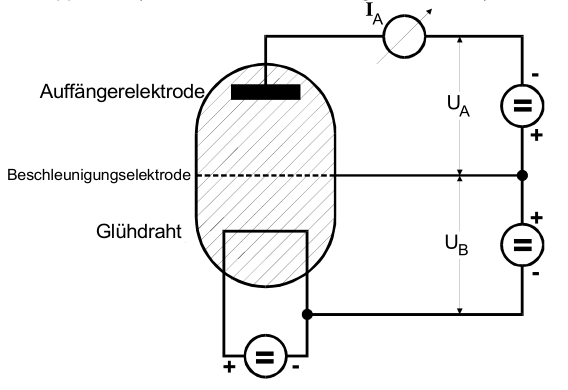
\includegraphics[width=0.7\textwidth]{latex/images/Aufbau.PNG}
            \caption{Schematischer Aufbau des Frank-Hertz-Versuches.}
            \label{img:aufb}
        \end{figure}

        \noindent Aufgrund des glühelektrischen Effekts treten nun Elektronen aus dem Draht aus, dieser Effekt wird dadurch verstärkt, dass ein 
        Oxid eines Erdalkalimetalles mit einer geringeren Austrittsarbeit auf den Draht aufgetragen wird. Zur Beschleunigung der Elektronen ist 
        gegenüber von dem Glühdraht eine netzförmige Elektrode mit einer positiven Gleichspannung $U_{\text{B}}$ welche die Elektronen auf eine 
        kinetische Energie des Betrags

        \begin{equation*}
            \frac{m_0 \cdot v_{\text{vor}}^2}{2} = \text{e}_0 U_\text{B}
        \end{equation*}

        \noindent beschleunigt. Bei der Formel wird jedoch nicht berücksichtigt, dass die Elektronen bereits eine Grundenergie besitzen können.
        Die beschleunigten Elektronen werden dann hinter der Elektrode an einer Auffängerelektrode aufgefangen, dadurch kann nun ein 
        Auffängerstrom $I_\text{A}$ gemessenen werden. Um jedoch eine Aussage über die Energie der Elektronen machen zu können besitzt die 
        Auffängerelektrode eine Gegenspanneng $U_{\text{A}}$ gegenüber der Elektrode, es entsteht ein Bremsfeld. Die Elektronen müssen also 
        eine gewisse kinetische Energie in z-Richtung
        
        \begin{equation*}
            \frac{m_0}{2} v_{\text{z}}^2 \geq \text{e}_0 U_{\text{A}}
        \end{equation*}

        \noindent besitzen um an der Auffängerelektrode anzukommen.
        Im Beschleunigungsraum ist aber auch der Quecksilberdampf, es kommt zu Zusammenstößen zwischen den Hg-Atomen und den Elektronen.
        Ist die Energie der Elektronen nicht groß genug, treten nur elastische Stöße auf. Da die Masse des Ag-Atoms ungefähr $1836 \cdot 201$ 
        größer ist ist ald die des Elektrons berechnet sich die abgegebene Energie nach 

        \begin{equation*}
            \Delta E = \frac{4 m_0 M}{\left(m_0 + M \right)^2} E \approx 1,1 \cdot 10^{-5} E
        \end{equation*}

        \noindent zu einem sehr geringem Wert. Die Richtung des Elektrons kann jedoch durch den elastischen Stoß deutlich verädert werden.\\
        Erreichen die Elektronen die Energie $\text{E}_1 - \text{E}_0$ der Energiedifferez zwischen dem Grundzustand und dem ersten angeregtem Zustand von HG, 
        stoßen die Elektronen nicht mehr elastisch mit den Hg-Atomen. Bei dem unelastischen Stoß übetragen die Elektronen dann ganau diese 
        Differenz an das Hg-Atom und behahalten die Energie $E - (\text{E}_1 - \text{E}_0)$. Innerhalb der Relaxationszeit geben die Quecksilber 
        Atome dann ein Lichtquant der Energie

        \begin{equation*}
            \text{h} \nu = \text{E}_1 - \text{E}_0 
        \end{equation*}

        \noindent ab. Hier ist h das Planksche Wirkungsquantum und $\nu$ die Frequenz des Lichtquants.
        Zur Untersuchung der Anregung des Hg-Atoms wird der Auffängerstrom $I_\text{A}$ in Abhängigkeit von der Beschleunigungsspannung $U_\text{B}$ 
        beobachtet. Mit steigender Beschleunigungsspannung $U_\text{B}$ steigt der Auffängerstrom solange bis die Energie der Elektronen 
        den Wert $\text{E}_1 - \text{E}_0$ erreichen. Wir diese Energie erreicht geben die Elektronen genau den Energiebetrag $\text{E}_1 - \text{E}_0$ 
        an die Hg-Atome ab und haben fast keine Geschwindigkeit mehr. Somit sind sie nicht mehr in der Lage das Bremsfeld zu durchqueren und der 
        Auffängerelektrode fällt abrupt auf 0 ab. Erst wenn die Beschleunigungsspannung weiter erhöt wird und die Elektronen wieder nach dem 
        Stoß genug beschleunigt werden um des Bremsfeld zu durchqueren, steigt auch wieder der Auffängerstrom an zu steigen. Dieses Verhalten 
        wiederholt sich dann regelmäßig mit steigender Beschleunigungsspannung und es bildet sich ein Kamm aus Strompeaks wie in Abbildung(\ref{img:Kamm})
        zu sehen ist. Die Spannungsdifferenz zwischen 2 dieser Peaks berechnet sich dann nach den Vorüberlegungen zu 

        \begin{equation*}
            U_1 := \frac{1}{\text{e}_0} \text{E}_1 - \text{E}_0 .
        \end{equation*}

        \noindent Somit lässt sich nun eine AUssage über die Energiedifferenz der ersten angeregten Zustände von Hg-Atomen.

        \begin{figure}[ht]
            \centering
            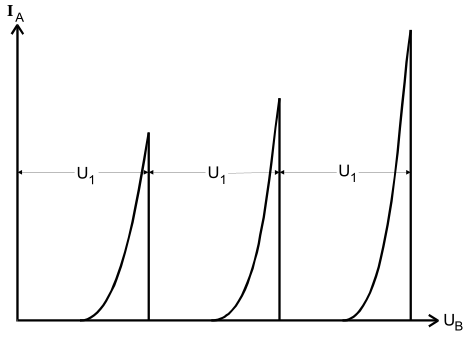
\includegraphics[width=0.7\textwidth]{latex/images/Kamm.PNG}
            \caption{Skizze einer optimalen Frank-Hertz-Experiment Kurve.}
            \label{img:Kamm}
        \end{figure}

    \subsection{Einfüsse auf die Gestalt der Franck-Hertz-Kurve}

        \noindent Die gemessene Kurve wird am ende jedoch nicht die Form von Abbildung(\ref{img:Kamm}) haben. Sie wird durch unterschiedliche Effekte 
        noch beeinflusst und verändert.

        \subsubsection{Kontaktpotential}

            \noindent Die Elektronen durchlafuen beim Beschleunigen ein Potentialgefälle(\ref{img:pot}) innerhalb des Glaskolbens, denn die Austrittsarbeiten der 
            Glükathode und der Beschleunigungselektrode sind nicht identisch. Hauptsächlich liegt das hier an der niedrigen Austrittsarbeit des 
            Glühdrahtes.

            \begin{figure}[ht]
                \centering
                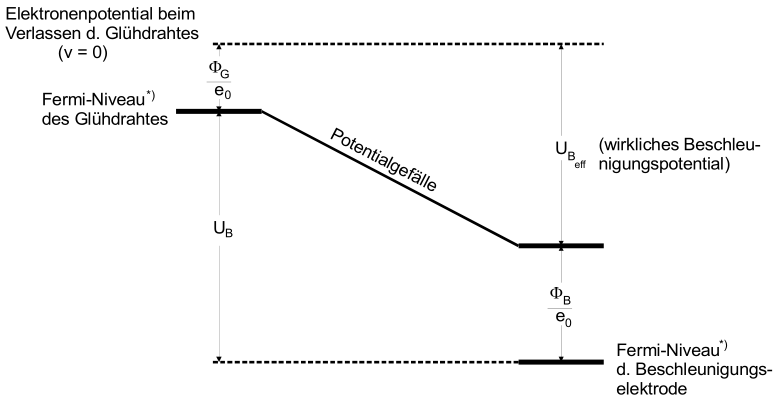
\includegraphics[width=0.7\textwidth]{latex/images/Kontaktpotential.PNG}
                \caption{Darstellung des Potentialgefälles welches zu dem Kontaktpotential führt.}
                \label{img:pot}
            \end{figure}

            \noindent Aus dem tatsächlichem Potentialgefälle kann dann die Beschleunigungsspannung $U_{\text{B,eff}}$ 
            
            \begin{equation*}
                U_{\text{B,eff}} = U_{\text{B}} - \frac{1}{\text{e}_0} ( \Phi_{\text{B}} - \Phi_{\text{G}})
            \end{equation*}

            \noindent berechnet werden.

            \noindent Hier wird der Ausrduck 

            \begin{equation*}
                K := \frac{1}{\text{e}_0} ( \Phi_{\text{B}} - \Phi_{\text{G}})
            \end{equation*}

            \noindent als Kontaktpotental bezeichnet.

        \subsubsection{Energieverteilung der Elektronen}

            \noindent Die durch den glühelektrischen Effekt frei werden Elektronen haben bereits eine kinetische Energie, diese ist auch nach 
            der Fermi-Dirac-Verteilung nicht diskret Verteilt, sondern kontinuirlich ausgebreitet. Durch diesen Effekt werden die theorischen 
            scharfen Kanten nach dem Abfallen des Auffängerstroms abgerundet, es entstehen eher Stromminima.

        \subsubsection{Einfluss des Dampfdruck}

            \noindent Der Dampfdruck gibt an wie dicht die Hg-Atome innerhalb des Kolben verteilt sind. Diese Dichte wird durch die mittlere 
            freie Weglänge $\bar{w}$ beschrieben und sollte für eine hohe Trefferwahrscheinlichkeit deutlich kleiner als der Abstand $a$ zwischen
            der Kathode under der Beschleunigungskathode sein.$\bar{w}$ kann durch den Sättigungsdampfdruck $p_{\symup{sät}}$ eingestellt werden, 
            nach der kinetischen Gastheorie ergibt sich 

            \begin{equation*}
                \bar{w} \quad [\text{cm}] \quad = \frac{0,0029}{p_{\symup{sät}}} \quad [p \text{ in mbar}] .
            \end{equation*}

            \noindent Der hier genutze Sättigungsdampfdruck lässt sich mittels der Dampfdruck-Kurve über die Temperatur nach der Gleichung 

            \begin{equation*}
                p_{\symup{sät}}(T) = 5,5\cdot10^{7} \text{exp}(-6876/T)  \quad (p \text{ in mbar, } T \text{ in K}) 
            \end{equation*}

            \noindent berechnen. Für eine ausreichende Stoßwahrscheinlichkeit $\bar{w}$ sollte 1000 bis 4000 mal größer als $a$ sein. 

        \subsubsection{Aufbau der Hg-Elektronenhülle}

            \noindent Die tatsächliche Energie des Übergangs wird dadurch verringert, dass das Umklappen des Elektronenspinns sehr 
            unwahrscheinich ist. Aus dem Grundzustand von n=6, S=0 und L=0 übergeht das Elektronen also nicht in den höher energetischen 
            Zustand n=7, S=0, L=0 des Singluett-System. Beobachtet wird der Übergang in einer der Zustäde des Triplett-Systems, diese sind in 
            Abbildung(\ref{Term}) zu sehen. Diese Stöße sind wahrscheinlicher da das Stoßelektron gegen einer der 6s Elektronen mit 
            entgegengesetztem Spin ausgetauscht wird.

            \begin{figure}[ht]
                \centering
                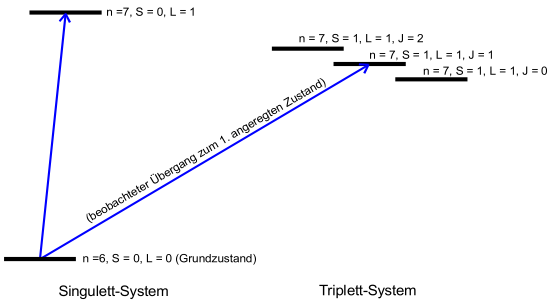
\includegraphics[width=0.7\textwidth]{latex/images/Singulett.PNG}
                \caption{Termschemades Hg-Atoms.}
                \label{img:Term}
            \end{figure}

    \subsection{Durchführung}

        \begin{figure}[ht]
            \centering
            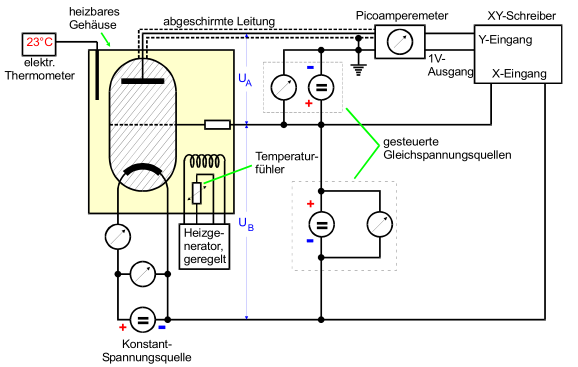
\includegraphics[width=0.7\textwidth]{latex/images/Schaltbild.PNG}
            \caption{Ein Schaltbild des des Versuchsaufbau zum Aufnehmen der Frank-Hertz-Kurve.}
            \label{img:Term}
        \end{figure}

        \noindent Zum Aufnehmen der Frank-Hertz-Kurve wird auf dem XY-Schreiber das Millimeterpapier befestigt. Um nun Werte aufnehmen zu können
        muss der Schreiber auf die jeweilige Messreihe angepasst werden, dazu können mit hilfe der Zero Räder die Achsen verschoben werben und 
        zusätzlich noch die Skallierung angepasst werden. Die erste Messreihe misst den Auffängerstrom in Abhängigkeit von der Bremsspannung, es 
        wird also die Beschleunigungsspannung konstant auf 11V gestellt. Dazu werden dann in 2 Teilen bei unterschiedlichen aber konstanten 
        Temperaturen die Bremsspannung variiert.
        Im zweiten Versuchsteil wird dann der Auffängerstrom in Abhängigkeit von der Beschleunigungsspannung gemessen. Jetzt wird die 
        Beschleunigungsspannung auf auf 1V gesetzt und bei einer Temperatur von 160-200$^\circ$C gemessen. 





        
        